\documentclass{article}
\usepackage{graphicx}
\usepackage{minted}


\title{SMBUD 2021 - Project work 1}
\author{\\Aman Gabba\\Andrea Cerasani\\Giovanni Demasi\\Pasquale Dazzeo\\Vlad Marian Cimpeanu}
\date{ \begin{figure}[b] \centering 
\includegraphics[scale=0.2]{Logo Polimi.png} \end{figure}
 }

\usepackage{ifxetex}
\usepackage{ifluatex}
\newif\ifxetexorluatex % a new conditional starts as false
\ifnum 0\ifxetex 1\fi\ifluatex 1\fi>0
   \xetexorluatextrue
\fi

\ifxetexorluatex
  \usepackage{fontspec}
\else
  \usepackage[T1]{fontenc}
  \usepackage[utf8]{inputenc}
  \usepackage[lighttt]{lmodern}
\fi

\usepackage{textcomp}
\usepackage{xcolor}
\usepackage{listings}
\usepackage{upquote}

\definecolor{keyword}{HTML}{2771a3}
\definecolor{pattern}{HTML}{b53c2f}
\definecolor{string}{HTML}{be681c}
\definecolor{relation}{HTML}{7e4894}
\definecolor{variable}{HTML}{107762}
\definecolor{comment}{HTML}{8d9094}

\lstset{
	numbers=none,
	stepnumber=1,
	numbersep=5pt,
	basicstyle=\small\ttfamily,
	keywordstyle=\color{keyword}\bfseries\ttfamily,
	commentstyle=\color{comment}\ttfamily,
	stringstyle=\color{string}\ttfamily,
	identifierstyle=,
	showstringspaces=false,
	aboveskip=3pt,
	belowskip=3pt,
	columns=flexible,
	keepspaces=true,
	breaklines=true,	
	captionpos=b,
	tabsize=2,
	frame=none,
}

\lstset{upquote=true}

\lstdefinelanguage{cypher}
{
	morekeywords={
		MATCH, OPTIONAL, WHERE, NOT, AND, OR, XOR, RETURN, DISTINCT, ORDER, BY, ASC, ASCENDING, DESC, DESCENDING, UNWIND, AS, UNION, WITH, ALL, CREATE, DELETE, DETACH, REMOVE, SET, MERGE, SET, SKIP, LIMIT, IN, CASE, WHEN, THEN, ELSE, END,
		INDEX, DROP, UNIQUE, CONSTRAINT, EXPLAIN, PROFILE, START, COUNT, IS, NULL
	}
}


\newcommand{\mycdots}{\cdot\!\cdot\!\cdot}
\lstset{language=cypher,
	literate=*
	{...}{$\mycdots$}{1}
	{theta}{$\theta$}{1}
}


\begin{document}

\maketitle
\thispagestyle{empty}

\newpage

\tableofcontents

\newpage

\section{Introduction}

\subsection{Problem Specification}
The aim of this project was to design a 'query graph data structure' in Neo4j for supporting a contact tracing application for COVID-19. The database must register all the necessary information about the users including vaccines and Covid swabs in order to have a pandemic trend overview for a given country. The application using this database will be able to exploit all the data coming from tracking applications and from all the public facilities.
\subsection{Hypothesis}
The assumptions taken into account are the following:

\begin{itemize}

\item People belonging to the same family live in the same house if not explicitly specified. Using the concept of "house" instead of "family", it is offered the possibility to differentiate domicile from residence.
\item All the personal data are verified by an authoritative figure, for instance the government.
\item The domicile declaration is assumed to be truthful.
\item All the data coming from public spaces are always considered true and complete.
\item People always provide all the necessary information to the staff when they visit a certain public space.
\item Every MEETS relationship is automatically added to the database by a tracing app when two mobile phones stay in the same range for more than 15 minutes. We assume that to every device corresponds only one person and viceversa.
\item Relationships use the Data type instead of Timestamp (with the exception of Test relationship because could happen that a person due to a positive resulting rapid test do in the same day another test which results negative - the use of Timestamp is important to recognise false positive) to register the relations because of safety and simplicity reasons. The former reason allows people using the Database to trace contacts during all the day and not only during a range of time (for more control). The latter reason is required due to avoid mistakes by the staff of public facilities during the time registration (an error in time registration could lead to a wrong tracing).
\item The designed model doesn't take into consideration the deaths, as the main focus of the project was the tracking of Covid infections. However in a more complete model that considers this aspect, a death node could be used to represent it through a dead relationship that connect the dead person to the death node with a date attribute. This choice could be useful to analyze the death/infection ratio related to the Covid pandemic.

\end{itemize}

\section{ER diagram}
The designed ER diagram contains the following entities: Person, Public Space, Vaccine, House and Covid Test. The other classes have been introduced due to ER diagram correctness reasons, but they haven't been taken into account during the design of the Graph Database because the last one allows a more flexible design. 

As said before the concept of 'Family' has been replaced with the concept of 'House' since it is more realistic and more useful for contact tracing.
\\
\\The Person entity has SSN ('Codice Fiscale' in Italy) as primary key and all the relevant data. Every Vaccine has its name and lot. Houses are described by a unique ID, address and town. 
Covid tests are identified by the timestamp and they also have the result as attribute. Every Public Space has name, city and strees as primary key and also a type attribute to identify its category.
Visits and Meeting entities, as said before, have been introduced due to correctness aspect but they are represented only as relationship in the graph diagram. Lives and Vaccines relationship are identified by date. 

\begin{figure}[h]
\centering 
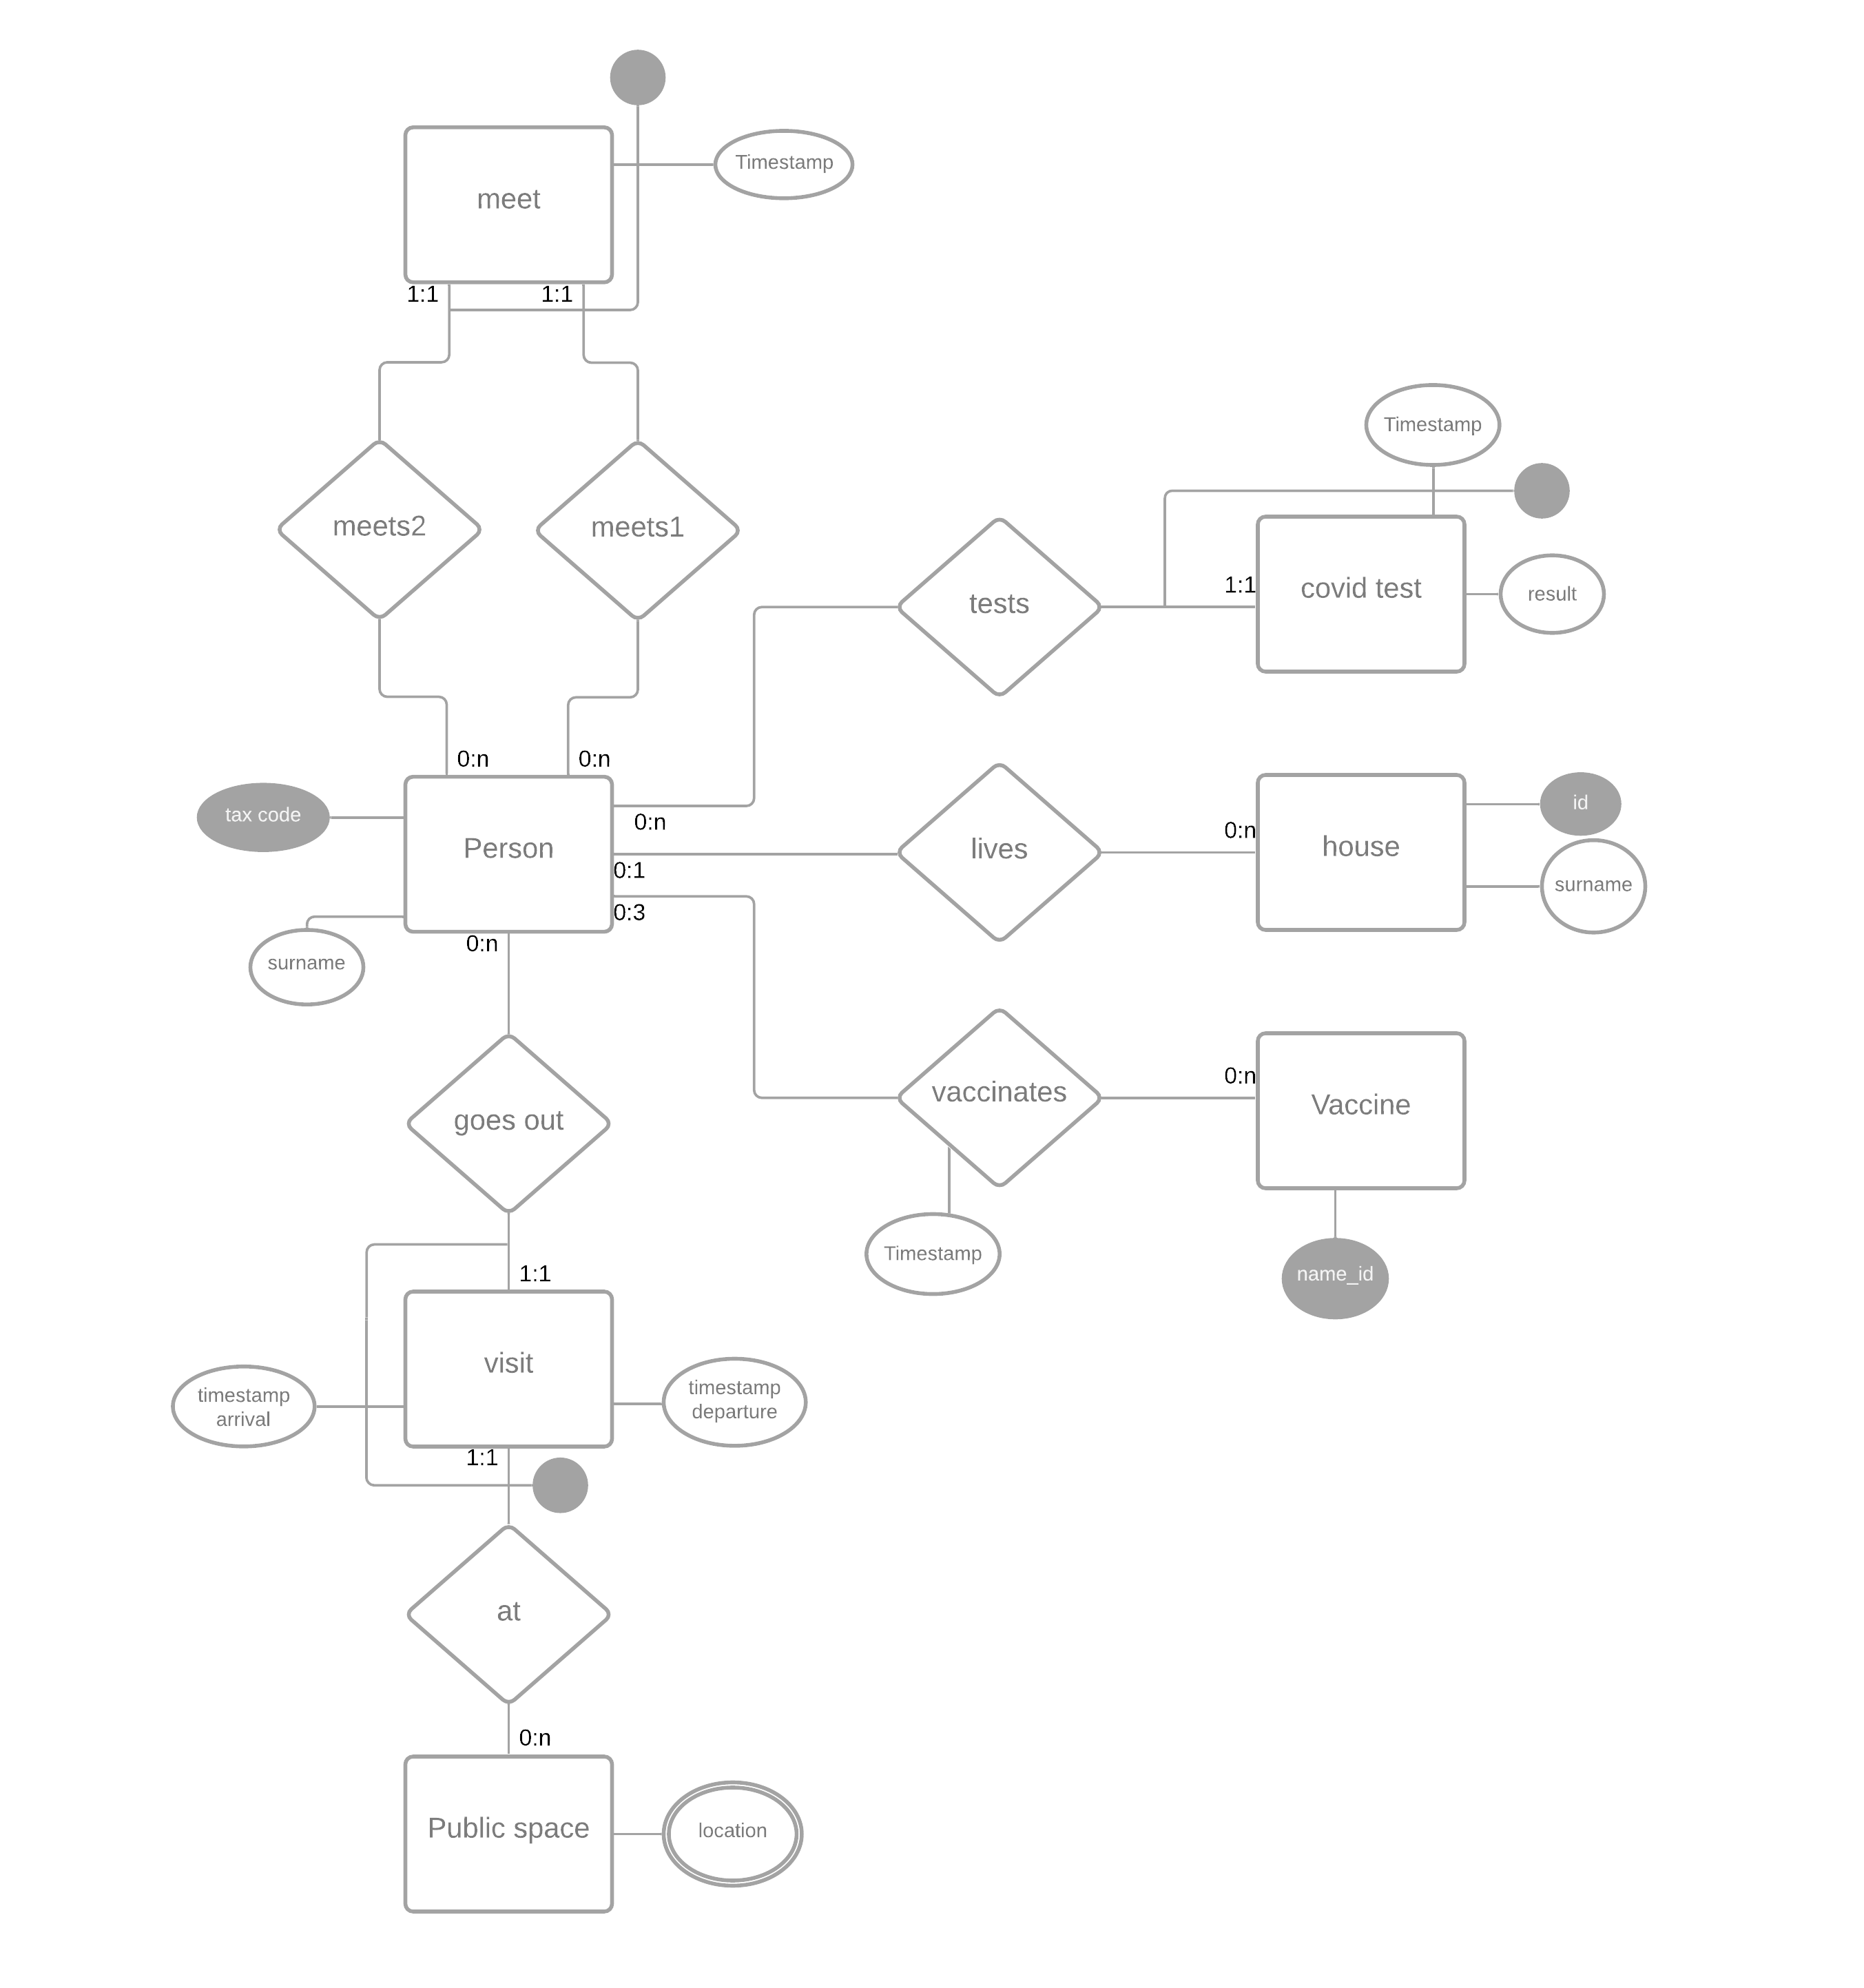
\includegraphics[scale=0.25]{er.png} 
\end{figure}
\newpage

\section{Graph diagram}
The designed Graph diagram is shown below. Person, House, Vaccine, Public Space and Covid Swab are represented as nodes and they all have the same attributes shown in the ER above. The relationship of the database are Meets, Lives, Tests, Vaccinates and Visits, they all have date as attribute (excepted tests that has timestamp). Vaccinate also has the lot of the vaccine and Tests also has the result of the test.

\begin{figure} [h]
\centering 
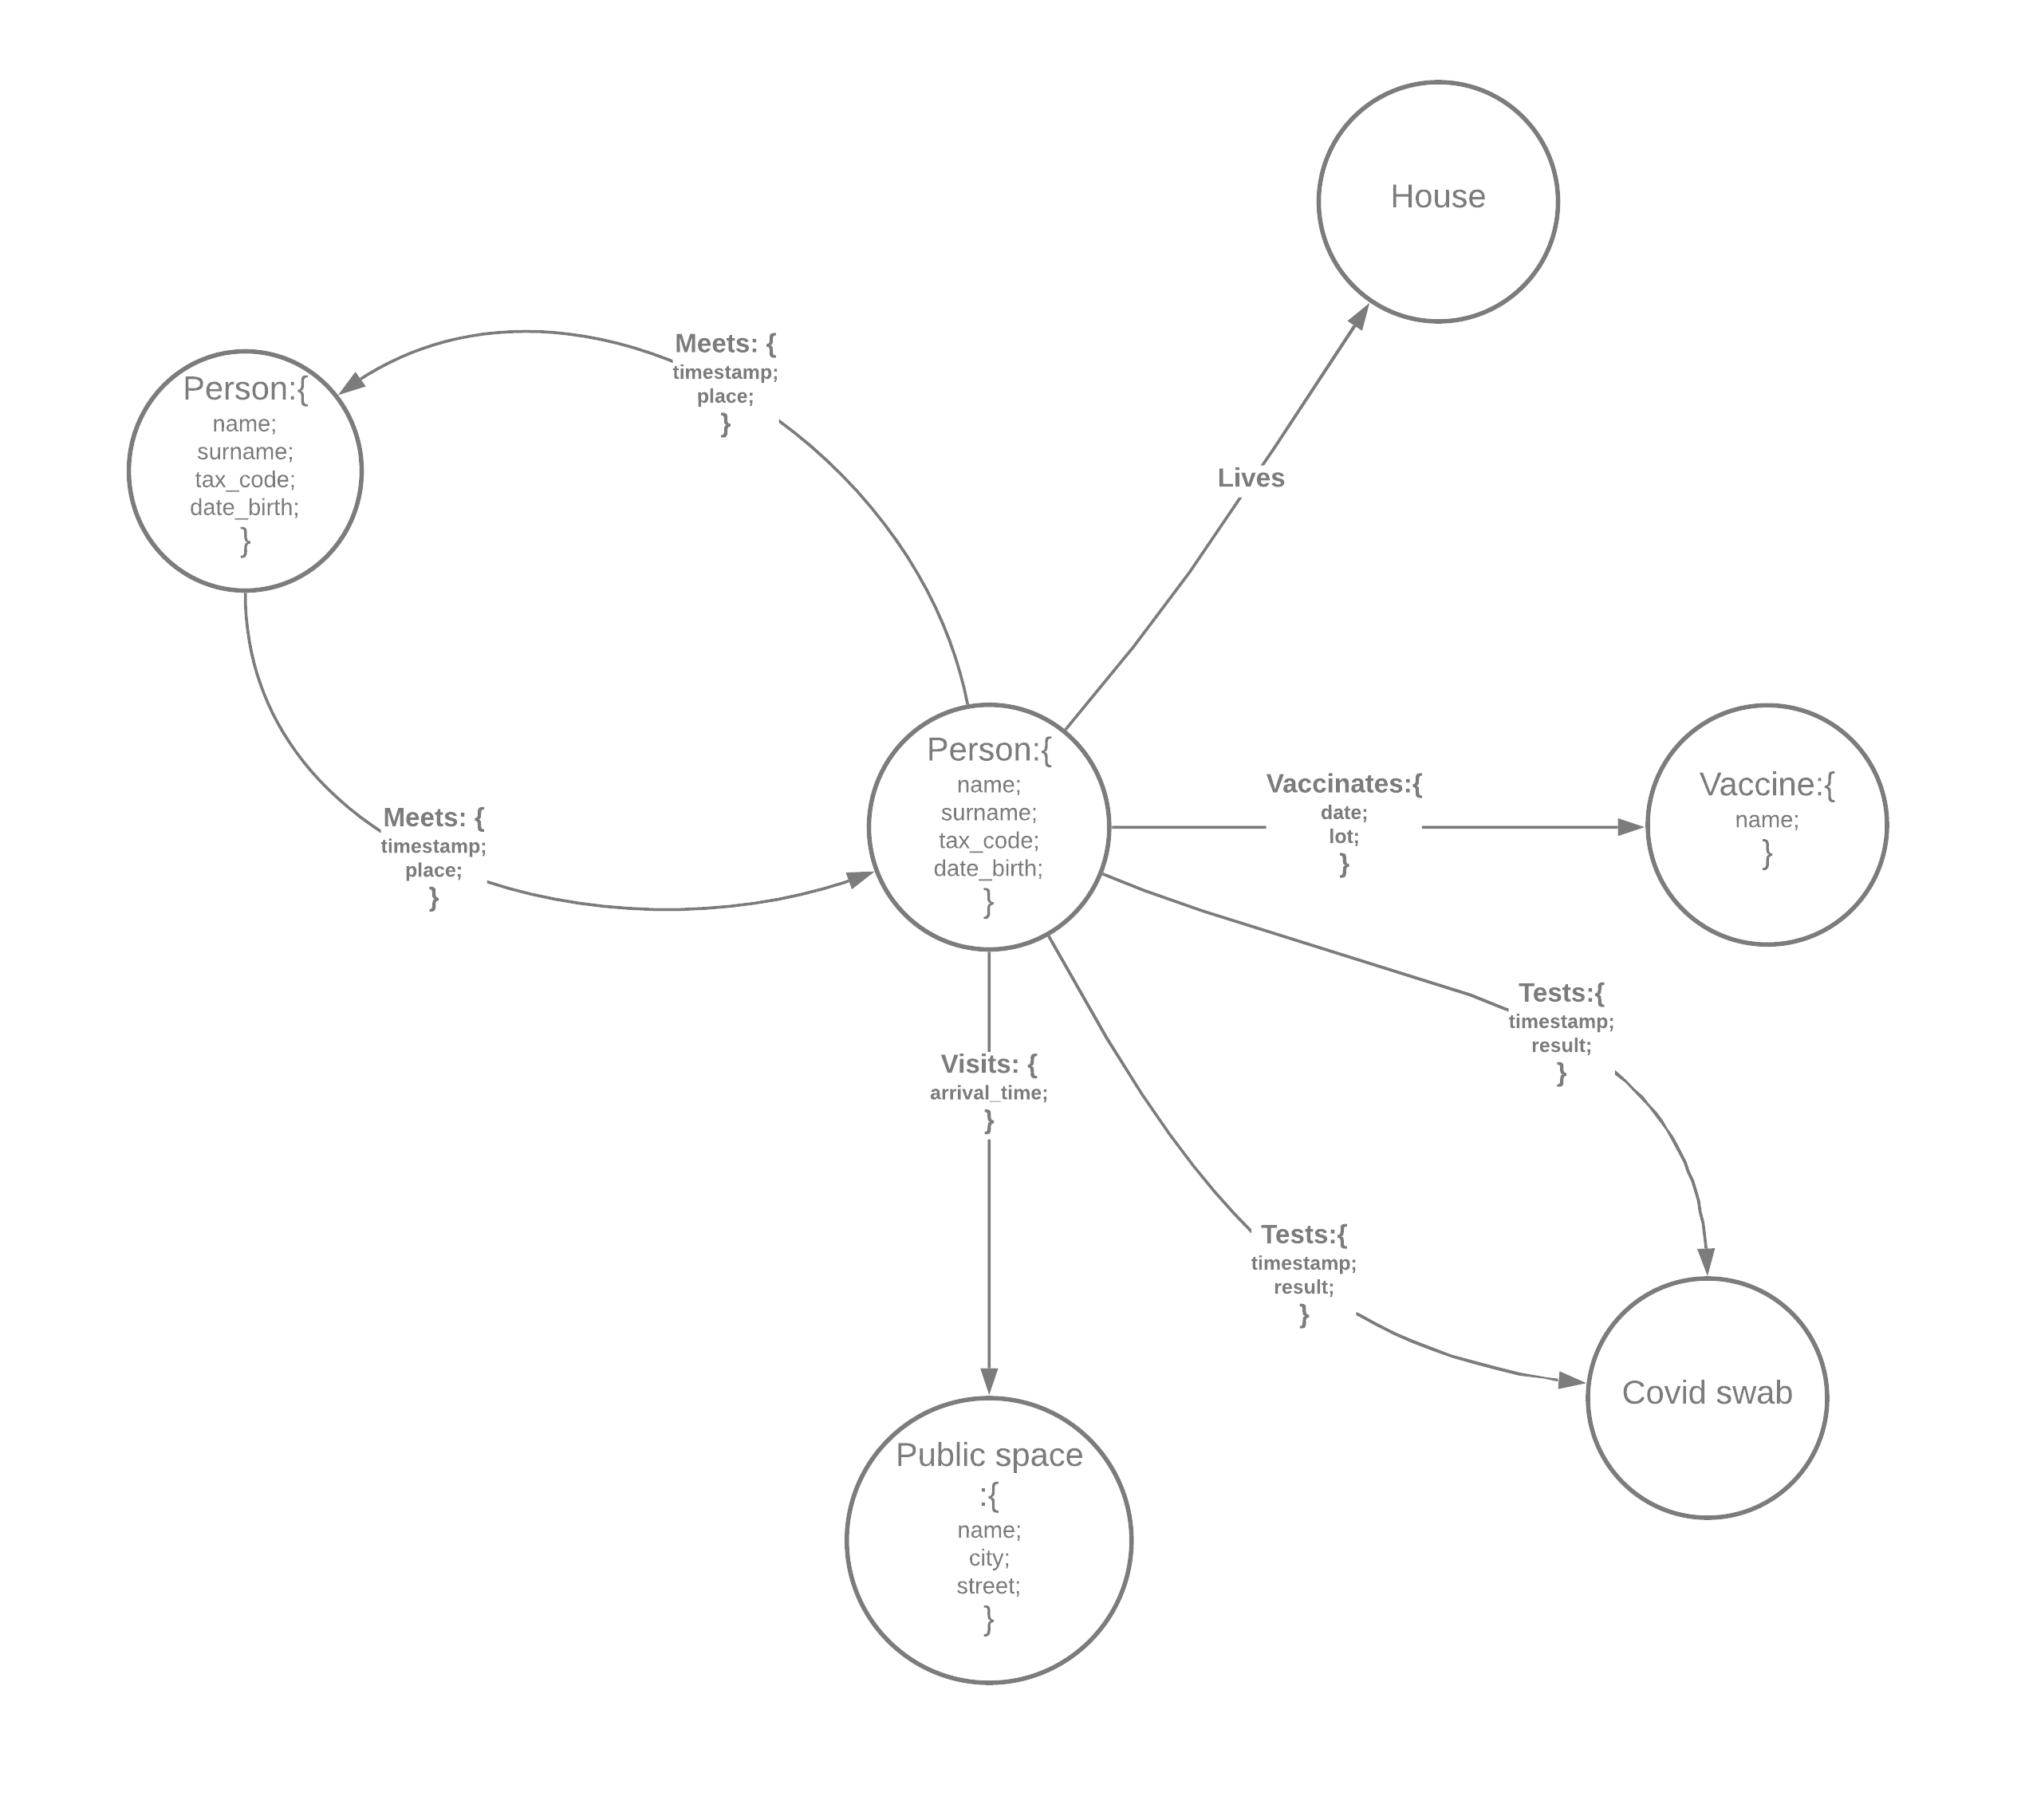
\includegraphics[scale=0.15]{Graph_diagram.png} 
\end{figure}
\newpage

\section{Dataset description}
The Dataset has been built by making a script in Python, using some useful packages like: random-italian-person that automatically generates people with random attributes (this package has been modified due to our necessity); the official binary Neo4j driver for Python for the communication with the Database since it allows to make queries directly from Python. 

\\
\hfill\break
We have also used this piece of code to generate amenities data. This query has been used in overpass turbo (a web-based tool for extracting OpenStreetMap data) selecting the map area of Rome, Naples and Milan.

\begin{lstlisting}[language=cypher, label=lst:cypher-example]

[out:csv("amenity","name", "addr:street", "addr:housenumber", "addr:city"; true; ",")]; 
// gather results 
( 
  //query part for: “amenity=post_box” 
  node"amenity"="restaurant"; 
  node"amenity"="bar"; 
  node"amenity"="cinema"; 
); 
// print results 
out body; 
>; 
out skel qt;
\end{lstlisting}
\newpage
\section{Queries and Commands}
\subsection{Queries}
\subsubsection{Vaccination percentage for a given age range}
The following query can be used to show the percentage of vaccinated people in an age range.
X and Y must be two positive integers with \$age\_min $\le$ \$age\_max.\\

\begin{lstlisting}[language=cypher, label=lst:cypher-example]
MATCH (sample: Person)
WHERE duration.between(date(sample.birthdate), date()).years >= $age_min
      AND
      duration.between(date(sample.birthdate), date()).years <= $age_max
WITH sample AS sizeSample
MATCH (vaccinated:Person)-[:VACCINATES]->(vaccine: Vaccine)
WHERE duration.between(date(vaccinated.birthdate), date()).years >=   
      $age_min
      AND
      duration.between(date(vaccinated.birthdate), date()).years <=   
      $age_max
RETURN 
CASE
WHEN COUNT(DISTINCT vaccinated) = 0 THEN 0.0
WHEN COUNT(DISTINCT sizeSample) = 0 THEN 0.0
ELSE (COUNT(DISTINCT vaccinated) * 1.0 / COUNT(DISTINCT sizeSample) * 1.0) * 100.0 
END AS Percentage

\end{lstlisting}
\subsubsection{Infection ratio per month}
Query that returns the infection ratio among all the tested people for each month.
\begin{lstlisting}[language=cypher, label=lst:cypher-example]

MATCH ()-[t:TESTS]->()
WITH date(apoc.date.format(apoc.date.parse(t.timestamp, 'ms', 'yyyy-MM-dd'), 'ms', 'yyyy-MM-dd')).month AS month,
     date(apoc.date.format(apoc.date.parse(t.timestamp, 'ms', 'yyyy-MM-dd'), 'ms', 'yyyy-MM-dd')).year AS year, count(t) as all_tests
OPTIONAL MATCH ()-[t:TESTS]->()
WHERE date(apoc.date.format(apoc.date.parse(t.timestamp, 'ms', 'yyyy-MM-dd'), 'ms', 'yyyy-MM-dd')).month = month AND
    date(apoc.date.format(apoc.date.parse(t.timestamp, 'ms', 'yyyy-MM-dd'), 'ms', 'yyyy-MM-dd')).year = year AND
    t.res = 'Positive'
RETURN round((COUNT(t) * 1.0 / all_tests * 1.0) * 100.0 * 100.0) / 100.0 AS ratio, month, year
ORDER BY year DESC, month DESC
\end{lstlisting}
\subsubsection{False positives}

The following query finds false positives (for false negatives it is necessary to switch pre with post in the last two lines before the Return statement).
\begin{lstlisting}[language=cypher, label=lst:cypher-example]

MATCH (p: Person)-[pre: TESTS]->()<-[post:TESTS]-(p)
WHERE duration.between(datetime({ epochMillis: apoc.date.parse(pre.timestamp, 'ms', 'yyyy-MM-dd HH:mm:ss')}), datetime({ epochMillis: apoc.date.parse(post.timestamp, 'ms', 'yyyy-MM-dd HH:mm:ss')})).hours < 24
AND duration.between(datetime({ epochMillis: apoc.date.parse(pre.timestamp, 'ms', 'yyyy-MM-dd HH:mm:ss')}), datetime({ epochMillis: apoc.date.parse(post.timestamp, 'ms', 'yyyy-MM-dd HH:mm:ss')})).hours > 0
AND post.res="Negative"
AND pre.res="Positive"
RETURN p, pre, post
\end{lstlisting}

\subsubsection{Most unsafe public spaces for a given city}
This query returns the infection ratio of every place of a desired city, in a selected year and month, as sum of people who became positive after being in a place over the total amount of visits of that place in the same period.
\$month and \$year are, respectively, the desider month and year and \$city is the city taken into consideration.
\begin{lstlisting}[language=cypher, label=lst:cypher-example]

MATCH (p1:Person)-[v:VISITS]->(ps:PublicSpace)
WHERE date(v.date).month = $month AND date(v.date).year = $year
      AND ps.city = $city
WITH ps.name AS space_name, v AS total_visits, p1 AS total_people
OPTIONAL MATCH (p:Person)-[t:TESTS]->()
WHERE p.ssn IN total_people.ssn AND t.res = 'Positive' AND duration.inDays(date(total_visits.date), date(apoc.date.format(apoc.date.parse(t.timestamp, 'ms', 'yyyy-MM-dd'), 'ms', 'yyyy-MM-dd'))).days >= 0 AND duration.inDays(date(total_visits.date), date(apoc.date.format(apoc.date.parse(t.timestamp, 'ms', 'yyyy-MM-dd'), 'ms', 'yyyy-MM-dd'))).days <= 15
RETURN
CASE
WHEN COUNT(DISTINCT p) = 0 THEN 0.0
ELSE (COUNT(DISTINCT p)*1.0 / COUNT(DISTINCT total_people)*1.0)*100.0
END AS percentage, space_name ORDER BY percentage DESC
\end{lstlisting}

\subsubsection{Vaccine efficacy}
This query can be used to analyze the Vaccine efficacy computed as the ratio of the vaccinated who became positive over the total number of vaccinated people.

\begin{lstlisting}[language=cypher, label=lst:cypher-example]

MATCH (p1:Person)-[:VACCINATES]->(v1:Vaccine {name: 'AstraZeneca'})
MATCH (p2:Person)-[:VACCINATES]->(v2:Vaccine {name: 'Moderna'})
MATCH (p3:Person)-[:VACCINATES]->(v3:Vaccine {name: 'Pfizer'})
MATCH (p4:Person)-[:VACCINATES]->(v4:Vaccine {name: 'Jensen'})
WITH COUNT(DISTINCT p1) AS vaccinated_astrazeneca, COUNT(DISTINCT p2) AS vaccinated_moderna, COUNT(DISTINCT p3) AS vaccinated_pfizer, COUNT(DISTINCT p4) AS vaccinated_jensen
OPTIONAL MATCH ()<-[t1:TESTS]-(p1:Person)-[v1:VACCINATES]->(vacc1:Vaccine {name: 'AstraZeneca'})
WHERE t1.res = 'Positive'
    AND date(apoc.date.format(apoc.date.parse(t1.timestamp, 'ms', 'yyyy-MM-dd'), 'ms', 'yyyy-MM-dd')) > date(v1.date)
OPTIONAL MATCH ()<-[t2:TESTS]-(p2:Person)-[v2:VACCINATES]->(vacc2:Vaccine {name: 'Moderna'})
WHERE t2.res = 'Positive'
    AND date(apoc.date.format(apoc.date.parse(t2.timestamp, 'ms', 'yyyy-MM-dd'), 'ms', 'yyyy-MM-dd')) > date(v2.date)                                       
OPTIONAL MATCH ()<-[t3:TESTS]-(p3:Person)-[v3:VACCINATES]->(vacc3:Vaccine {name: 'Pfizer'})
WHERE t3.res = 'Positive'
    AND date(apoc.date.format(apoc.date.parse(t3.timestamp, 'ms', 'yyyy-MM-dd'), 'ms', 'yyyy-MM-dd')) > date(v3.date)
OPTIONAL MATCH ()<-[t4:TESTS]-(p4:Person)-[v4:VACCINATES]->(vacc4:Vaccine {name: 'Jensen'})
WHERE t4.res = 'Positive'
    AND date(apoc.date.format(apoc.date.parse(t4.timestamp, 'ms', 'yyyy-MM-dd'), 'ms', 'yyyy-MM-dd')) > date(v4.date)
WITH vaccinated_astrazeneca,vaccinated_moderna,vaccinated_pfizer,vaccinated_jensen, COUNT(DISTINCT p1) AS vaccinated_infected_astra, COUNT(DISTINCT p2) AS vaccinated_infected_moderna, COUNT(DISTINCT p3) AS vaccinated_infected_pfizer, COUNT(DISTINCT p4) AS vaccinated_infected_jensen
RETURN (1- (toFloat(vaccinated_infected_astra)/toFloat(vaccinated_astrazeneca)))*100 AS AstraZenecaEfficacy,
    (1- (toFloat(vaccinated_infected_moderna)/toFloat(vaccinated_moderna)))*100 AS ModernaEfficacy,(1- (toFloat(vaccinated_infected_pfizer)/toFloat(vaccinated_pfizer)))*100 AS PfizerEfficacy,(1- (toFloat(vaccinated_infected_jensen)/toFloat(vaccinated_jensen)))*100 AS JensenEfficacy
\end{lstlisting}

\subsubsection{People to quarantine}
This query returns all the people a given person has been in contact with in the last 15 days. In detail it returns all the people met by a given person in the last 15 days (incubation period) from a given date with the tracking app, his/her family and all the people that have been in the same place during the same day as him/her.
The following query can be used to find all the people who need to be put in quarantine due to a positive test of the given person.
\$fiscal\_code is the fiscal code of the person receiving the vaccine (16 digits alphanumeric code), \$end\_date is the last day of the incubation period (\$incubation).

\begin{lstlisting}[language=cypher, label=lst:cypher-example]

MATCH (infected:Person)-[l1:LIVES]->(h)<-[l2:LIVES]-(person:Person)
WHERE infected.ssn = $fiscal_code
  AND date(l1.livesFrom) <= $end_date AND (date(l1.movingDate) >= $end_date - $incubation OR l1.movingDate is  NULL)
  AND date(l2.livesFrom) <= $end_date AND (date(l2.movingDate) >= $end_date - $incubation OR l2.movingDate is NULL)
  AND (date(l2.movingDate) >= date(l1.livesFrom) OR date(l2.livesFrom) <= date(l1.movingDate))
RETURN person
UNION
MATCH (infected: Person)-[v1:VISITS]->()<-[v2:VISITS]-(person: Person)
WHERE infected.ssn = SSN AND v1.date = v2.date AND duration.inDays(date(v1.date), date(XXX)).days <= 15 AND duration.inDays(date(v1.date), date(XXX)).days >= 0
RETURN person
UNION
MATCH (infected: Person)-[m:MEETS]->(person: Person)
WHERE infected.ssn = SSN AND duration.inDays(date(m.date), date(XXX)).days <= 15 AND duration.inDays(date(m.date), date(XXX)).days >= 0
RETURN person
\end{lstlisting}

\subsection{Commands}
\subsubsection{New vaccination}
The following command can be used to add a vaccination. \$ssn is the fiscal code of the person receiving the vaccine (16 digits alphanumeric code), \$vax\_name is the name of the vaccine ('AstraZeneca', 'Jensen', 'Pfizer', 'Moderna'), \$lot is the lot of the vaccine (it must must be in format AZ\#\#, P\#\#,J\#\#,M\#\#). \$vax\_date is the date of the vaccination and must be in the following format YYYY-MM-DD.

\begin{lstlisting}[language=cypher, label=lst:cypher-example]

MATCH (person_to_vaccinate: Person),
      (vax: Vaccine)
WHERE person_to_vaccinate.ssn = $ssn
      AND 
      vax.name = $vax_name
CREATE (person_to_vaccinate)-[:VACCINATES {lot: $lot, 
        date: $vax_date}]->(vax)
        
\end{lstlisting}
\subsubsection{New Covid Test}
The following command can be used to add a Covid Test. \$ssn is the fiscal code of the person tested (16 digits alphanumeric code), \$result is the result of the test ('Positive' or 'Negative'). \$timestamp is the timestamp of the test and must be in the following format 'YYYY-MM-DD hh:mm:ss'.

\begin{lstlisting}[language=cypher, label=lst:cypher-example]

MATCH (person_tested: Person),
      (test: Swab)
WHERE person_tested.ssn = $ssn 
      AND 
      test.name = 'Covid Swab'
CREATE (person_tested)-[:TESTS {res: $result, timestamp: $timestamp}]->(test)

\end{lstlisting}
\subsubsection{Moving a family}
The following query changes all the LIVES relations of the people who live in the same house by adding them a movingDate attribute and makes new relations with the new house (this command could be useful in case of moving family).
\$ssn is one of the people who lives in the old house. \$id is the id of the new house (Integer number) and \$moving\_date is the date of the moving and it must be in the following format YYYY-MM-DD.


\begin{lstlisting}[language=cypher, label=lst:cypher-example]

MATCH (p1:Person)-[l1:LIVES]->(h:House)
WHERE p1.ssn = $ssn AND l1.movingDate IS NULL
WITH h AS old_house
MATCH (p2:Person)-[l2:LIVES]->(old_house)
WHERE l2.movingDate IS NULL
WITH p2 as people_moving, l2
MATCH (h:House) WHERE ID(h) = $id
CREATE (people_moving)-[:LIVES{livesFrom: $moving_date}]->(h)
SET l2.movingDate = $moving_date

\end{lstlisting}

\newpage

\section{Generator database}
The {\fontfamily{qcr}\selectfont"neo4jDB-populator/main.py"} file is responsible of generating a random database.
In order to correctly run the generator, it is mandatory to store the Neo4j password in {\fontfamily{qcr}\selectfont"Neo4jDB-populator/password.txt"}, in this way the generator will be able to connect with the database.
\\This script exploits the following packages: pandas, numpy, neo4j and python-codicefiscale.

\subsection{Cities generation}
This generator will create data for the following cities: Rome, Milan and Naples. For each city it will create nodes representing public spaces available in that specific town.

\subsection{People generation}
In order to consistently generate people, it was decided to assign a number of houses per city, by default the number of houses per city is set to 15. Every time an house is built, the generator will also create a family of 'Person' to link to that house.
Each family randomly consists of 1 to 6 members.

\subsection{Relationships generation}
For improving the quality information extracted from the data, people living in a certain city must "VISITS" only public spaces of the same city, and for the same reason, people can "MEETS" people of the same city with 90\% of probability.
In order to get significant results from queries, the number of "VISITS" relations was set to 1 visit per person every 3-5 days. This setting may impact on the generation data-set time, indeed it could take up to 1-2 minutes to generate all the data.


\section{Application description}
Goal of the application {\fontfamily{qcr}\selectfont"GUI/App.py"} is to give some information about the pandemic.
The user can use the application in order to know about:
\begin{itemize}
    \item Trend Covid: the application will display the ratio of positive people among all the tests carried out per each month.
    \item Vaccine efficacy: the application will display how many people vaccinated with a specific vaccine has been negative over all
    the people vaccinated with the same vaccine.
    \item Dangerous places: selected a specific city, the user can see which are the most dangerous public spaces in that city. The danger level of
    a given public space is calculated as the percentage of people that tested positive after 15 or less days, and then is normalized considering
    all the other public places: in this way the most dangerous public space will have a danger level of 1,
    whereas the less unsafe place will have a danger level equal to 0.
    \item Vaccinates per age: the application will display the percentage of people vaccinated per each age range.
    The age range considered are [20,29], [30,39], [40, 49], ..., [90, 100].
\end{itemize}

\section{User guide}
The application is meant to work on pc or macOS. As the application has been entirely developed in Python, it is not
operative system dependent.
In order to correctly run the application it is mandatory to store the Neo4j password in {\fontfamily{qcr}\selectfont"neo4jDB-populator/password.txt"},
in this way the application will be able to connect with the database.
\\The user must check to have installed correctly in the virtual environment the following packages: {\fontfamily{qcr}\selectfont tkinter,
matplotlib, pandas, neo4j, numpy and python-codicefiscale}.

\newpage

\section{Conclusion}

Some interesting conclusions can be drawn from the development of this project: Graph databases are, if well designed, easy to use and really scalable. \\
The creation of credible databases using Python could be really convenient to simulate a real situation and understand in advance which behaviours could be useful to manage the situation in exam.\\
Graph databases are more flexible than the classical relational databases since they allow to create same situations in an easier and more realistic way.

\section{References and Sources}
\begin{itemize}
    \item Random-italian-person package: https://pypi.org/project/random-italian-person
    \item Neo4j package: https://neo4j.com/docs/python-manual/current
    \item Tkinter package: https://docs.python.org/3/library/tkinter.html
    \item Overpass turbo API: https://wiki.openstreetmap.org/wiki/Overpass\_API
\end{itemize}



\end{document}
